\documentclass[a4paper,12pt,oneside,openany]{report}
\usepackage{layout}
\setlength{\textwidth}{15.0 cm}
\setlength{\textheight}{25.0 cm}


\usepackage[english,brazil]{babel}
\usepackage{pagina}	% pagina-padrao
\usepackage{indentfirst}		% for indent
\usepackage[utf8]{inputenc}
\usepackage{graphics,epsfig}
\usepackage{graphics}
\graphicspath{{./Figuras/}}
\usepackage{pstricks,pst-node,pst-tree}
\usepackage{alltt}
%\usepackage{makeidx}
%\makeindex
\usepackage[figuresright]{rotating} % for saydways tables and figures
\usepackage{enumerate}			% for configuration of enumerate environment
\usepackage{amsmath}
\usepackage{amssymb}
\usepackage{portland,multirow}

\setcounter{secnumdepth}{3}	% numeracao ate subsubsecao
\setcounter{tocdepth}{2}	% indice ate subsubsecao

\usepackage{longtable}
 

\begin{document}

\begin{center}
\textbf{UNIVERSIDADE FEDERAL DO RIO DE JANEIRO}
\vspace{-0.2cm}

\textbf{ESCOLA POLITÉCNICA}
\vspace{-0.2cm}

\textbf{DEPARTAMENTO DE ENGENHARIA ELETRÔNICA E DE COMPUTAÇÃO}
\vspace{0.8cm}

\underline{\textbf{PROPOSTA DE PROJETO DE GRADUAÇÃO}}

Aluno: Bruno Machado Afonso
\vspace{-0.2cm}

bruno.ma@poli.ufrj.br

Orientador: Mariane Rembold Petraglia
\end{center}

\textbf{1. TÍTULO}

Desenvolvimento de Base de Dados para Treinamento de Redes Neurais de Reconhecimento de Voz através da Geração de Áudios com Resposta
Ao Impulso Simuladas por Técnicas de Data Augmentation.

\vspace{0.4cm}
\textbf{2. ÊNFASE}

Computação

\vspace{0.4cm}
\textbf{3. TEMA}

O tema do trabalho é sobre o estudo de uma forma de simular Respostas ao Impulso de Ambientes Acústicos (RIR) com parametrizações diferentes a partir de amostras 
de RIR gravadas em ambientes reais, e ainda usar a RIR para gerar amostras de áudio em locais simulados a partir de gravações de voz reais.

\vspace{0.4cm}
\textbf{4. DELIMITAÇÃO}

O estudo é focado em inferir uma técnica de reforço de dados tanto em amostras reais de RIR quanto nas gravações de voz. Este trabalho está delimitado em apenas 
modificar amostras reais de áudio, e não gerar amostras simuladas sem uma gravação de base.

\vspace{0.4cm}
\textbf{5. JUSTIFICATIVA}

Com o avanço das tecnologias de automação residencial, assistentes pessoais nos smartphones e comunicação online, o estudo de técnicas de
processamento de áudio (no caso específico deste trabalho, relacionados a voz), tornou-se mais relevante para a sociedade.
Uma das características mais importantes a ser detectada no processamento de áudio é a Resposta ao Impulso de salas, 
que representa o modelo acústico do ambiente, pois através desta é possível extrair informações pertinentes do local em que o áudio foi gravado
e também detectar a posição de fontes sonoras e as isolar para reconhecimento.
No âmbito da área de reconhecimento de voz, a fala reverberante, ou seja, o sinal de fala combinado com o modelo acústico do ambiente
é um dos desafios encontrados para a detecção da voz, tornando a identificação do RIR de vital importância para o reconhecimento de fala \cite{FAR-FIELD_ASR}.

Junto a isso, houve avanços no âmbito do aprendizado de máquina, fornecendo alternativas para os métodos tradicionais
de processamento de áudio \cite{ML_Speech_Rec}.
Modelos de arquitetura de redes neurais necessitam de um grande volume de dados para que sejam treinados e aprimorados, e um dos mais recentes
desafios nessa área é o fato das bases de RIR não serem extensas, conforme esclarecidas no artigo \cite{Estimation_RT_DRR},
pois realizar uma grande quantidade de gravações de áudio é uma tarefa de alto custo tanto financeiro quanto temporal, necessitando de equipamento especializado
e diversos locais com características de modelo sonoro diferentes e pessoas diversas para amostras de voz.


\vspace{0.4cm}
\textbf{6. OBJETIVO}

O objetivo deste trabalho é desenvolver um algoritmo capaz de gerar amostras de RIR simuladas para diferentes ambientes a partir de uma RIR real e
gerar um banco de dados de amostras de voz convoluídas com as RIR simuladas e com ruídos para uso em treinamento de redes neurais.
Dessa forma, têm-se como objetivos específicos:

\begin{enumerate}
      \item Propor um algoritmo que altere as características da RIR para simular diferentes ambientes com RIR diferentes;
      \item Elaborar um algoritmo que faça o acréscimo de ruídos pontuais ou ruídos de fundo em uma amostra de voz;
      \item Desenvolver um sistema computacional que aplique ambos os algoritmos anteriores em sequência para gerar
      amostras de voz em ambientes ruidosos.
\end{enumerate}

\vspace{0.4cm}
\textbf{7. METODOLOGIA}

Um sinal de voz gravado em um ambiente pode ser interpretado como a junção de três partes: uma amostra de voz pura, sem nenhum fator externo
ou reverberação envolvido, convoluída com a Resposta ao Impulso da sala (RIR) onde ocorre a gravação, somada a um sinal de ruído, podendo este 
ser pontual ou um ruído de ambiente. A RIR representa um modelo acústico do ambiente, que define como um receptor acústico irá receber caso o áudio
seja gerado e percebido de dentro deste ambiente. Uma definição de Resposta ao Impulso é a de uma função que registra a pressão sonora temporalmente
em um ambiente fechado após uma excitação extremamente curta e cheia de energia (impulso de Dirac).

Neste trabalho é proposta uma forma de gerar RIR simuladas partindo de uma RIR real, ou seja, gravando um áudio que representa um impulso em um ambiente
fechado real, e alterando suas propriedades. Reproduz-se o que foi proposto no artigo de data augmentation para respostas ao impulso para
estimação do modelo acústico \cite{RIR_Data_Aug}, onde são geradas RIRs simuladas, modificando-se as propriedades de Tempo de Decaimento (T60) e de
razão entre áudio direto e reverberado (DRR). Através dessas duas propriedades, define-se praticamente todas as RIRs possíveis de serem gravadas
artificialmente.

Para gerar as amostras de vozes reverberadas que compõe a base de dados, acompanha-se o que é proposto no artigo de estudo de data
augmentation em vozes reverberadas \cite{Speech_Rec}, onde são convoluídos sinais de voz anecoicos com as RIRs simuladas que foram geradas anteriormente.
Além disso, é acrescentado a esse sinal de voz reverberado ruídos diversos, que são caracterizados de duas formas: ruídos pontuais e de ambiente.
Os ruídos pontuais são amostras de áudio curtas que podem ser introduzidos em qualquer momento da fala; já os ruídos de ambiente são sons constantemente
presentes ao fundo da gravação para simular um ambiente externo. Os ruídos foram extraídos da biblioteca MUSAN \cite{noiseLib}.

Através desses dois passos, são gerados vários sinais de vozes reverberados artificialmente. A simulação da RIR tem por objetivo colocar
a amostra de voz em vários ambientes fechados, e a inclusão de ruídos ajudam drasticamente no treinamento de redes neurais, impedindo que as redes fiquem
viciadas em características muito específicas da fala durante o treinamento, uma vez que eles tendem a simular os fatores
externos que podem estar envolvidos em uma gravação real.

%\vspace{0.4cm}
\pagebreak
\textbf{8. MATERIAIS}

\begin{itemize}
      \item Computador:
      \begin{itemize}
            \item CPU: Arquitetura amd86, AMD Ryzen 3600X 3.8GHz
            \item RAM: 16 GB RAM DDR4
            \item HDD: 1 TB
      \end{itemize}

      \item Software:
      \begin{itemize}
            \item MATLAB\textregistered \space R2018a (Software não-gratuito, requer licença para uso)
            \item ITA-Toolbox, plugin open source para medições acústicas para MATLAB\textregistered
      \end{itemize}

      \item Dados:
      \begin{itemize}
            \item The Aachen Impulse Response (AIR) Database \cite{AIR_Database}, base de dados com respostas ao impulso
            gravadas de diferentes ambientes.
            \item MUSAN: A Music, Speech, and Noise Corpus \cite{noiseLib}, base de dados com amostras de ruídos pontuais
            e ruídos de fundo.
      \end{itemize}
\end{itemize}

\pagebreak

\begin{figure}[htp]      
      \begin{center}
      \makebox[\textwidth]{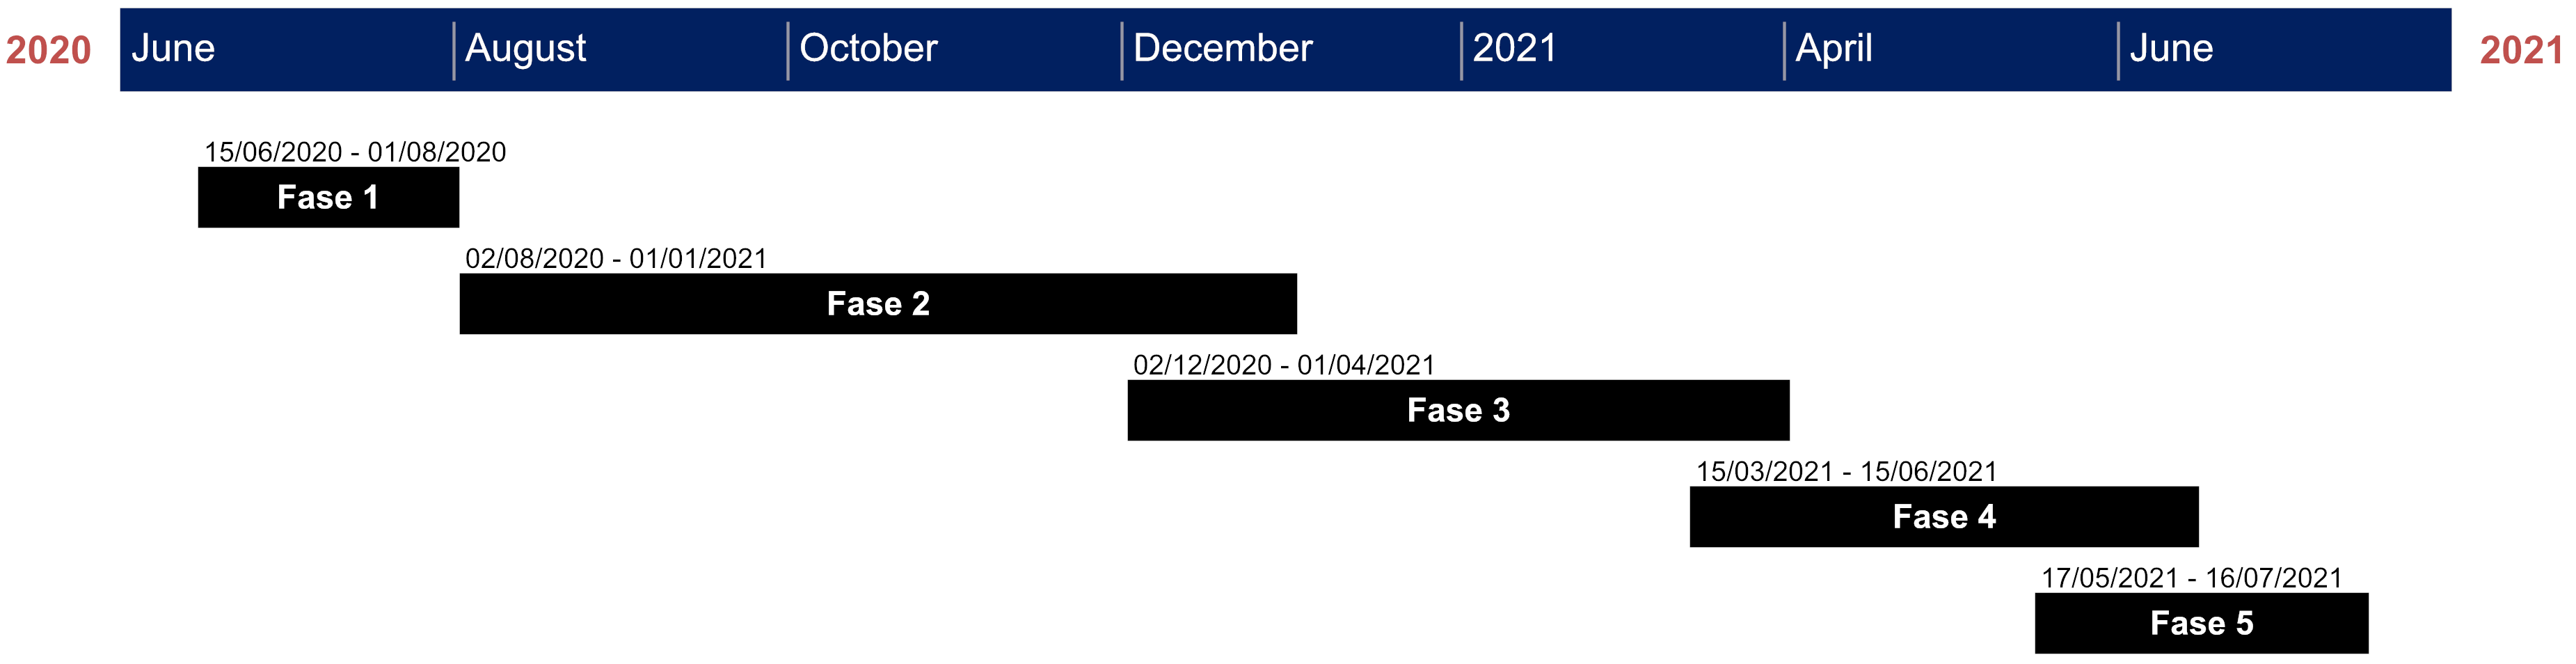
\includegraphics[width=1.35\textwidth]{cronograma-bruno.png}}
      \caption{\footnotesize{Cronograma do projeto}}
      \label{Fig:Cronograma}
      \end{center}
\end{figure} 

\vspace{0.4cm}
\textbf{9. CRONOGRAMA}

Apresentado graficamente conforme a Figura \ref{Fig:Cronograma}.

Fase 1: Estudo sobre a Resposta ao Impulso sonoro e sobre os seus principais parâmetros.

Fase 2: Desenvolvimento e implementação do algoritmo proposto \cite{RIR_Data_Aug} de reforço de dados para as RIR.

Fase 3: Desenvolvimento e implementação do algoritmo proposto \cite{Speech_Rec} de incremento de ruídos pontuais e de fundo em amostras de voz.

Fase 4: Desenvolvimento e implementação do algoritmo que cria sinais de voz com RIR e ruídos gerados nas etapas anteriores.

Fase 5: Escrita do texto do projeto de graduação.


\bibliography{TCC_Proposta_bib} 
\bibliographystyle{ieeetr}

\vspace{2cm}
\noindent
Rio de Janeiro, 7 de junho de 2021

\vspace{0.5cm}
\begin{flushright}
      \parbox{10cm}{
      \hrulefill

      \vspace{-.375cm}
      \centering{Bruno Machado Afonso - Aluno}

      \vspace{0.9cm}
      \hrulefill

      \vspace{-.375cm}
      \centering{Mariane Rembold Petraglia - Orientadora}

      \vspace{0.9cm}
      }
\end{flushright}
\vfill
      
\end{document}
